% !TEX program = xelatex
\documentclass[12pt,a4paper]{ctexart}

% ---------- Packages ----------
\usepackage{geometry}
\geometry{left=2.5cm,right=2.5cm,top=2.5cm,bottom=2.5cm}
\setlength{\headheight}{15pt}

\usepackage{graphicx}
\usepackage{booktabs}
\usepackage[hidelinks]{hyperref}
\usepackage{caption}
\usepackage{float}
\usepackage{setspace}
\onehalfspacing

\usepackage{fancyhdr}
\pagestyle{fancy}
\fancyhf{}
\fancyhead[C]{利维坦如何改变自然状态：基于元胞自动机的计算实验}
\fancyfoot[C]{\thepage}
\renewcommand{\headrulewidth}{0.4pt}

% ---------- Metadata ----------
\title{{\bfseries 利维坦如何改变自然状态\\[4pt] ——基于元胞自动机的计算实验}}
\author{}
\date{}

\begin{document}
\maketitle

\vspace{-8pt}

\begin{abstract}
\noindent
霍布斯在《利维坦》中描述的自然状态——没有共同权力约束所有人时，人的生活将陷于持续的恐惧与暴力——其核心机制能否通过计算模型加以检验，至今仍是政治哲学与计算社会科学之间的开放问题。本文以元胞自动机为工具，在二维网格上模拟囚徒困境中的空间演化博弈，比较自然状态下合作自发涌现的轨迹与集中化惩罚机制（利维坦）引入后的轨迹变化。实验覆盖五个背叛诱惑强度（$b \in \{1.2, 1.4, 1.6, 1.8, 2.0\}$）与三个惩罚强度（$p \in \{0.1, 0.3, 0.5\}$），每组参数重复五次以计算统计量。核心发现是，利维坦在 $b=1.6$ 时效果最为显著——合作率从约 42\% 跃升至约 73\%——但在 $b \ge 1.8$ 时完全失效。这意味着集中化惩罚只能在合作已有脆弱基础的条件下改变演化走向，它无法凭空创造秩序。本文的贡献不在于重复论证“利维坦是否必要”，而在于为霍布斯的论证提供了一个可观测的动力学框架：利维坦不是均衡的保证者，而是轨迹的催化剂。

\vspace{6pt}
\noindent{\bfseries 关键词}：霍布斯；利维坦；元胞自动机；空间演化博弈；囚徒困境；合作涌现
\end{abstract}

% ======================================================================
\section{引言}
% ======================================================================

1651年，霍布斯在《利维坦》中做出了政治哲学史上最令人不安的预测之一：在没有一个共同权力威慑所有人的“自然状态”中，任何人的安全都无法得到保障。即使两个人都不想打仗，他们也“无法很好地相互信任”——因为“A 没有理由不相信 B 会先下手”。因此，自然状态是一种持续的战争状态。霍布斯的解决方案是利维坦，一个垄断暴力的主权者，通过对背叛者的惩罚来保证契约履行。

从哲学论证的角度看，霍布斯的推理链条是严密的。但从经验研究的角度看，这组命题留下了一系列尚未充分展开的问题。自然状态中的合作到底能不能自发产生，哪怕是局部或暂时的？如果可以，它在什么条件下会扩张，又在什么条件下会崩溃？利维坦的引入不是简单地把自然状态“关掉”，而是与一个已经运行了一段时间的演化系统发生交互——那么，这个交互过程本身是什么样的？这些问题指向同一个方向：霍布斯描绘的不是一个均衡的比较（有利维坦 vs.\ 没有利维坦），而是一个演化过程，而传统博弈论在比较均衡时恰好忽略了这个过程。

本文试图用计算模型来部分地填补这个缺口。具体做法是把囚徒困境放在一个二维空间网格上，让每个个体只与其空间邻居互动，按“模仿收益最高者”的规则逐轮更新策略。这个框架——即 Nowak \& May (1992) 开创的空间演化博弈——使我们可以观察合作与背叛在空间中的此消彼长，而不是仅仅计算它们最终各占多少比例。在此基础上，我们在演化的中途（第500步）引入一个集中化的惩罚机制（利维坦），对背叛者施加固定罚分，然后观察演化轨迹如何——或是否——因此改变。

选择元胞自动机而不是解析方程模型或基于 agent 的随机模拟，是出于研究问题本身的特点。元胞自动机的演化规则完全透明：每个时间步的每个策略更新都可以追溯。这种透明性对本文的目的至关重要，因为它允许读者检验从霍布斯的哲学概念到计算变量之间的映射是否合理——如果某一步出了偏差，那是映射的问题，不是“模型内部不可解释”的问题。此外，空间局部互动与霍布斯自然状态中“个体并非与所有人互动，而是与邻居互动”的隐含假设相符。

本文其余部分的结构如下。第二节综述霍布斯自然状态的博弈论解释和空间演化博弈的方法论传统，指出直接比较“利维坦中途引入前后”的演化轨迹是一个文献缺口。第三节明确从霍布斯的哲学概念到计算变量的映射关系，区分一一对应、代理指标和近似三类关系。第四节详述模型设定与实验设计，参数选择的每一步都给出文献依据或理论理由。第五节报告实验结果。第六节讨论这些结果对霍布斯理论的含义和模型本身的边界。第七节总结。

% ======================================================================
\section{文献综述与理论框架}
% ======================================================================

\subsection{霍布斯自然状态的博弈论形式化}

把霍布斯的自然状态转化为博弈论模型时，面临的首要问题不是”用什么参数”而是”选哪种博弈”——囚徒困境还是确信博弈。这个选择直接决定利维坦的角色应该被建模为惩罚机制还是协调机制。

囚徒困境（Prisoner's Dilemma, PD）的支持者——Taylor (1976, 1987) 和 McLean (1981)——抓住了霍布斯叙述中的一个核心要素：在自然状态中，不论对方怎么选，先发制人总是更安全的选择。在 PD 中，背叛是严格占优策略，这与霍布斯”每个人都被迫先下手”的逻辑具有结构上的同构性。McLean 进一步从超博弈角度指出，霍布斯关于”力量大致平等”的假设——自然状态中”最弱者也有足够的能力杀死最强者”——使得个体无法通过武力优势跳出困境，因而陷入了囚徒困境式的集体非理性。

确信博弈（Assurance Game / Stag Hunt）的支持者提出了一个重要的反驳。Moehler (2009) 的论证基于霍布斯的第二自然法和第三自然法：第二自然法要求每个人都”愿意寻求和平”，第三自然法要求”履行契约”。Moehler 由此推断，霍布斯的自然状态不是个体理性与集体理性冲突（PD 的结构），而是相互信任的缺失——“如果每个人确信他人也会履约，合作就是理性的”。换言之，自然状态的根本问题不是利益冲突，而是协调失败。Skyrms (2004) 从演化博弈的角度支持了这一立场，论证许多社会契约场景——包括霍布斯的原始契约——从结构上看更接近 Stag Hunt。

这两种立场对利维坦应该做什么有截然不同的含义。在 PD 框架下，利维坦需要通过惩罚来改变收益结构，使合作成为相对更好的选择。在 Assurance 框架下，利维坦的作用更接近于一个”焦点”——它发出可信的信号，使所有人都预期他人会合作，从而协调到合作的均衡上。

本文选择 PD 框架，理由有两条。第一，PD 的”背叛严格占优”结构与霍布斯第十三章对自然状态的本体论描述一致——自然状态中的人不是”不确定要不要合作”，而是”有充分理由不合作”。第二，正因为 PD 中合作不是均衡，利维坦的效果才更值得检验：如果惩罚能在背叛占优的环境中创造合作，它在更宽松的博弈结构中只会更强而不是更弱。在第六节，我们会回到这个选择，讨论 Assurance 框架下的替代预期。

\subsection{空间演化博弈：从随机配对到空间邻居}

Nowak \& May (1992) 在二维网格上的模拟——用他们自己的话说——发现了一个”反直觉的”结果。在随机配对的囚徒困境中，合作毫无疑问会灭绝：背叛占优，演化向全员背叛收敛。但当他们把个体放在网格上、让每个个体只与最近邻互动时，合作者通过形成紧密的空间集群存活了下来。集群内部的合作者互给高收益，集群边缘的合作者虽然被背叛者剥削，但集群整体作为一个”空间堡垒”向内补偿了边缘的损失。

这一发现的关键参数是背叛诱惑强度 $b$。Nowak \& May 使用简化 PD 参数化（$R=1, T=b, P=S=0$），在 $b \in (1, 2]$ 范围内观察到了三个行为区间：$b < 1.8$ 时合作者形成稳定的空间集群；$1.8 < b < 2.0$ 时为动态共存，合作与背叛形成不断变化的迷宫图案；$b > 2.0$ 时合作者无法维持。这个相变结构对本文的实验设计至关重要：$b=1.8$ 附近的临界行为决定了自然状态”有多严酷”，也因此决定了利维坦发挥作用的空间有多大。

后续研究对更新规则和网络结构做了扩展。Szab\'{o} \& T\H{o}ke (1998) 比较了确定性模仿最优与随机费米函数更新，发现后者的动力学更丰富——噪声的引入使系统可以在亚稳态之间跃迁，而不是锁定在一个确定性的空间模式中。Szab\'{o} \& F\'{a}th (2007) 的综述涵盖了二维网格、随机图、小世界网络和无标度网络上的合作演化，核心发现是：空间结构（或更一般地，群体结构）几乎总是比完全混合的群体更有利于合作。Ohtsuki \& Nowak (2008) 从演化图论角度提出了一个简洁的规则：当收益-成本比超过网络的平均度时，自然选择就有利于合作。这些发现共同构成了本文的方法论基础——元胞自动机不是研究合作的”好用的工具”，而是在数学上抓住了空间局部性对合作演化的核心作用。

\subsection{利维坦的建模传统}

Gross et al.\ (2016) 在《科学报告》上发表的行为实验是本文最重要的经验参照。他们在重复公共物品博弈中发现，参与者不仅可以维持合作，而且可以通过自愿将惩罚权委托给他人来维持合作——他们称这个过程为”建造利维坦”。关键发现是，自愿委托（而不是被分配）惩罚权对合作维持有独立贡献：控制组中惩罚权被外生分配的群体合作率仍然下降，但实验组中\textbf{选择}将惩罚权集中化的群体保持了高合作率。

Sigmund et al.\ (2010) 的理论分析补充了这一发现。他们比较了两种惩罚制度：分散化惩罚（每个合作者都可以惩罚背叛者，即 peer punishment）与集中化惩罚（惩罚资源被汇入一个公共池，由集体执行，即 pool punishment）。集中化惩罚在抑制二阶搭便车方面更有效——在分散化惩罚中，不愿意实施惩罚的合作者可以搭那些愿意实施惩罚的合作者的便车，而集中化惩罚通过制度设计规避了这个问题。

Grim, Mar \& St.\ Denis (2002) 代表了另一个相关的传统：用计算工具来研究哲学问题。他们的《哲学计算机》展示了元胞自动机、神经网络和遗传算法如何为经典的哲学难题——包括囚徒困境、社会契约和合作演化——提供新的视角。本文在方法论语境上承接了这个传统。

\subsection{本文的位置}

上述三条线索之间的一个空白是：没有人系统地比较过“利维坦在中途引入”前后的演化轨迹。Nowak \& May 的框架只有无惩罚的演化；Gross 等人的实验只有“一直有惩罚”和“一直没有惩罚”的比较；Sigmund 等人的模型分析的是惩罚制度本身的演化稳定条件。但是，霍布斯的叙事恰恰预设了一个先后顺序——人们先在自然状态中遭受苦难，然后才建立利维坦。如果利维坦不是从一开始就存在，而是在演化的中途被引入，它对轨迹的改变是否与“一开始就有惩罚”相同？如果不是，中途引入揭示的是利维坦的什么特征？本文的实验设计正是围绕这个问题构建的。

% ======================================================================
\section{概念映射}
% ======================================================================

在进入模型设定之前，有必要明确从哲学文本到计算变量之间的映射关系——哪些概念有一一对应关系，哪些只是代理指标，哪些是粗略的近似。这种透明性的意义在于，它划定了后续所有实验结论的诠释学边界：如果某条映射被判定为“近似”而非“一一对应”，那么基于该映射的推论就需要相应的保留。

下面的列表给出了八组核心映射。每组映射的判定标准是：如果霍布斯本人看到了这个变量及其在模型中的行为，他是否能够合理地将它与自己的概念对应起来？

\begin{enumerate}
  \item 自然状态中的个体被映射为元胞（一一对应）。每个元胞代表一个理性个体，Hobbes 的“力量平等”假设通过使所有元胞共享相同的收益矩阵来实现——没有内在的能力差异或资源禀赋差异。

  \item 相互提防（diffidence）被映射为相邻元胞中背叛者的比例（代理指标）。“恐惧”作为一种心理状态本身不可直接测量，但每个元胞所处的局部环境——周围有多少背叛者——可以在模型中精确计算，并作为个体是否感到受威胁的代理。

  \item 先发制人（anticipation）被映射为背叛策略在空间中的扩散过程（结构对应）。在模型中，当一个合作者被背叛者包围时，它面临两种选择：保持不变（收益持续被剥削）或转为背叛（至少不再单向受损）。当背叛从高密度区域向合作区域扩散时——即防御性背叛在空间中传播——这个过程在结构上对应了霍布斯“每个人都被迫先下手”的逻辑。

  \item 契约（covenant）被映射为稳定的合作集群（近似）。合作集群不等于法律契约，因为契约涉及承诺、义务和共同知识，而集群仅仅是合作者的空间聚集。但合作集群可以视为契约的\textbf{行为后果}——霍布斯认为契约创造了信任，信任促进了合作，因此合作集群在模拟中的出现标记了契约可能发生的空间位置。这个映射是近似的而非一一对应的，在解释结果时需要注意。

  \item 利维坦被映射为集中化惩罚机制（一一对应）。模型中的利维坦是一个全局规则，对所有背叛者施加固定的惩罚 $p$，没有选择性，也没有被惩罚者反制利维坦的可能。这个设计对应了霍布斯所描述的利维坦的核心特征：垄断暴力、统一执法。

  \item 自然状态被映射为无惩罚的 PD 演化（近似）。模拟捕捉了霍布斯自然状态的\textbf{核心结构特征}——无外部约束下的自利互动——但省略了霍布斯叙述中的历史细节（如美洲“野蛮人”的例子）和规范性维度。

  \item 和平被映射为合作均衡（代理指标）。在模型中，“和平”被操作化为合作者占绝对多数（$f_c > 0.85$）并持续保持在那个水平。但合作行为的高比例是和平的必要条件而非充分条件——在霍布斯的理论中，和平还需要制度基础（法律、司法、执法），而不只是行为的统计分布。

  \item 战争状态被映射为全员背叛或碎片化共存（代理指标）。$f_c$ 趋近 0 或者合作与背叛在空间中以迷宫模式进行持久拉锯战，这两种模式分别对应霍布斯“所有人对所有人的战争”和“冷战争”——没有大规模战斗但人人自危的自然状态。
\end{enumerate}

一个在解释实验结果时需要反复回到的区分是：本文测量的是\textbf{合作行为}而非\textbf{制度}。霍布斯的论证路径是制度先于行为——人们通过社会契约建立主权者，主权者制定法律，法律约束行为。但在计算模型中，我们观察的是合作行为在惩罚机制引入前后的涌现模式，模型中没有“契约”或“法律”的本体论地位。这种“行为先行、制度后置”的建模路径与霍布斯的哲学路径之间存在张力，但这恰恰是计算建模的价值所在——它允许我们在不预设制度存在的情况下，观察制度的功能等价物（惩罚机制）对行为的因果效应。

% ======================================================================
\section{模型设定与实验设计}
% ======================================================================

\subsection{元胞自动机的动力学}

模型的基础是一个 $100 \times 100$ 的二维方格，边界条件为周期边界（即网格的上边缘与下边缘相接，左边缘与右边缘相接，消除边界上的异常行为）。这种设定等价于在环面上进行模拟，在大样本下与无限网格的定性行为一致。

每个元胞在任意时刻持有两种策略之一：合作（C，编码为 1）或背叛（D，编码为 0）。初始状态为 50\% 合作者和 50\% 背叛者，随机分布在网格上。这个中性初始条件意味着每条模拟轨迹都从相同的出发点开始：一个没有任何空间结构、完全随机混合的合作-背叛分布。任何随后出现的空间模式——集群、迷宫、界面——都是从这种随机分布中\textbf{涌现}出来的，而不是被初始条件预设的。

每个时间步包含两个阶段：博弈与更新。

在博弈阶段，每个元胞与其 Moore 邻域中 8 个邻居（上下左右及四个对角）各进行一次囚徒困境博弈。收益矩阵采用 Nowak \& May (1992) 的简化参数化：

\begin{center}
\begin{tabular}{c|cc}
& 对方合作（C） & 对方背叛（D） \\
\midrule
我方合作（C） & $R=1$ & $S=0$ \\
我方背叛（D） & $T=b$ & $P=0$ \\
\end{tabular}
\end{center}

在这个参数化中，合作者对另一个合作者产生双方各得 1 的正和结果；合作者对背叛者产生合作者得 0 而背叛者得 $b$ 的转移；两个背叛者相遇则双方无所得。背叛诱惑强度 $b$ 是唯一变化的博弈参数，控制着“背叛相对合作的吸引力”。$b$ 越接近 1，合作与背叛的收益差越小，合作越容易存活；$b$ 越接近 2，单次博弈中背叛的优势越大，合作越难维持。

累计收益的计算很简单。一个元胞与 8 个邻居各玩一局 PD，将其从 8 局中获得的收益相加。合作者的总收益等于其 Moore 邻域（不含自身）中合作者的数量——因为与每个合作邻居玩得 1 分，与每个背叛邻居玩得 0 分。背叛者的总收益等于 $b$ 乘以邻域中合作者的数量——与每个合作邻居玩得 $b$ 分，与每个背叛邻居玩得 0 分。$b$ 的作用由此清晰可见：它决定了背叛者从每一个合作邻居身上提取多少额外收益。

在更新阶段，每个元胞检查自己及其 Moore 邻域中全部 9 个元胞的累计收益，下一轮采用其中收益最高者的策略。这就是 Nowak \& May 的“确定性模仿最优”规则。如果出现平局——即多个邻居收益相同且都是最高——元胞保持当前策略不变。这个平局规则将“自我”放在了优先位置，意味着要改变策略，必须有一个严格更好的邻居作为榜样；仅仅同样好还不够。更新是同步的：所有元胞在同一时刻切换到新策略，不存在异步更新中的策略传播时序效应。

\subsection{利维坦的建模}

在条件 B 中，利维坦被建模为一种集中化的惩罚机制，在第 500 步时被激活。其运作方式非常简洁：从第 500 步开始，每个背叛者的收益在原有基础上减去一个固定值 $p$。$p$ 的取值来自 Gross et al.\ (2016) 的实验发现——惩罚强度需要足够大才能改变行为，但多大的“足够大”取决于具体的社会困境结构。本文选取三个水平以覆盖从弱到强的范围：$p = 0.1$（弱惩罚，仅抵消 $b$ 带来的优势的一小部分），$p = 0.3$（中等惩罚），$p = 0.5$（强惩罚，使合作-背叛收益差在 $b \le 1.5$ 的范围内发生符号逆转）。

有两点值得说明这个设计为什么是“外生的”。第一，利维坦在第 500 步被引入，这个时间点不由元胞选择——不论当时的合作水平如何，利维坦都按时到来。第二，惩罚资源由利维坦自身承担——不存在合作者需要“纳税”来维持利维坦的二阶公共物品问题。外生设计的代价是牺牲了与 Gross et al.\ (2016) 的直接可比性（他们的核心发现恰恰是自愿委托是关键的），但收益是干净的因果推断：条件 A 与条件 B 在 $t \in [0, 499]$ 范围内使用相同的随机种子，生成的轨迹完全相同，只在 $t=500$ 处分叉。任何此后出现的差异都可以归因于利维坦的存在与否。

选择第 500 步作为引入点，背后的考虑是让自然状态有足够的时间“充分展开”。对于 $b=1.2$ 和 $b=1.4$，200 步以内合作集群就已经形成并趋于稳定，500 步时系统已经在一个稳态附近波动。对于 $b=1.6$，500 步处于动态共存的中间阶段——合作者与背叛者已经建立了各自的领地，但边界仍在持续推移。对于 $b=1.8$ 和 $b=2.0$，500 步时合作已经或几乎灭绝。在同一个时间点引入利维坦，我们可以观察它对这些处于\textbf{不同演化阶段}的系统各产生什么效果。

\subsection{参数空间的文献依据}

\begin{table}[H]
\centering
\caption{实验参数一览}
\begin{tabular}{@{}lll@{}}
\toprule
参数 & 取值 & 文献依据 \\
\midrule
$b$ & 1.2, 1.4, 1.6, 1.8, 2.0 & Nowak \& May (1992) 的完整相变区间 \\
$p$ & 0.1, 0.3, 0.5 & Gross et al.\ (2016) 的有效惩罚范围 \\
网格大小 & $100 \times 100$ & 平衡计算成本与空间模式分辨率 \\
邻域类型 & Moore (8) & Nowak \& May 标准设定 \\
更新规则 & 模仿最优 & Nowak \& May 确定性规则 \\
初始合作率 & 50\% & 中性初始条件 \\
总时间步 & 1000 & 500 步自然状态 + 500 步利维坦 \\
重复次数 & 5 & 蒙特卡洛均值与标准差 \\
\bottomrule
\end{tabular}
\end{table}

$b$ 值的选取覆盖了 Nowak \& May (1992) 报告的全部三个行为区间。$b=1.2$ 和 $b=1.4$ 属于合作者形成稳定集群的低诱惑区间；$b=1.6$ 位于中间地带；$b=1.8$ 是临界点的最近邻；$b=2.0$ 代表了背叛占优的极端情况。这个选取不是均匀间隔的——它在 $b=1.6$ 和 $b=1.8$ 之间更密，因为这里是系统行为发生质变的相变区间。

$p$ 值的选取需要单独说明。Gross et al.\ (2016) 的实验使用的是真实货币激励，惩罚对应于被试收入的直接扣除。在他们的设置中，有效的惩罚大约占禀赋的 10\%--50\%。我们将这个比例转化为本文简化参数化中“收益减去惩罚”的对应关系。$p=0.1$ 相当于每个背叛邻居只“损失”0.1 个单位的净收益——在 $b=1.2$ 时，背叛者的净收益从 $1.2 \times n_c$ 降为 $1.2 \times n_c - 0.1$，这只是一个微弱的抑制。$p=0.3$ 和 $p=0.5$ 则在较大范围内改变了背叛的吸引力。这三个值覆盖了从“几乎无效”到“显著有效”的预期范围，其间距也足够大，使我们能够区分不同惩罚强度的效果。

网格大小从 Nowak \& May 原版的 $200 \times 200$ 缩减为 $100 \times 100$ 是出于实际的计算约束。在 100 次运行（两个条件、五个 $b$ 值、三个 $p$ 值，各重复五次，外加快照收集）的总量下，$100 \times 100$ 将单次运行控制在 0.4--0.5 秒，使完整实验可以在不到一分钟内完成。100 的网格边长对应 10,000 个元胞，足以展示合作集群的形成、扩张和崩溃——Nowak \& May 在他们自己的稳健性检验中证实，$50 \times 50$ 以上的网格在定性行为上与更大网格一致，仅临界值的精确位置有轻微偏移。

\subsection{三个分析层次与指标}

实验的分析框架由三个递进的层次组成。这三个层次不是三个不同的实验，而是对同一组模拟数据的三种观察角度，每个角度对应一个霍布斯式的理论问题。

第一个层次关心的是合作是否能够出现——这是对霍布斯“自然状态中合作不可能”这一断言的最直接检验。对应的计算指标是：全局合作者比例 $f_c(t)$ 的时间序列、合作集群的数量、以及首次稳定集群形成时间 $\tau_e$——定义为 $f_c(t)$ 首次连续 100 步超过 5\% 的时间点。

第二个层次关心的是合作出现后能否扩张——对应霍布斯关于“相互提防阻止合作扩大”的论述。这里测量的是最大连通合作集群的面积 $A_{\max}(t)$（占全网格的比例）、合作-背叛界面的密度 $\rho(t)$（相邻的 C-D 对占总邻接对的比例，反映“前线”竞争强度），以及集群扩张速度 $dA_{\max}/dt$。

第三个层次关心系统的最终归宿——自然状态最终停留在战争还是和平？利维坦能否将系统推向合作均衡？这一层用最后 500 步的平均合作率 $f_c^\infty$ 作为稳态表征，用滚动标准差首次降至阈值以下的时间标记收敛速度，并将每个稳态分类为四种类型之一：全员合作（$f_c^\infty > 0.85$）、集群共存（$f_c^\infty \in [0.15, 0.85]$ 且最大集群面积 $>0.3$）、碎片化共存（$f_c^\infty \in [0.15, 0.85]$ 且最大集群面积 $\le 0.3$）、或全员背叛（$f_c^\infty < 0.05$）。

\subsection{研究假设}

基于上述模型设定和已有文献，本文提出三条假设，每条假设都对应一组可检验的定量预期。

\textbf{H1（自然状态下的合作涌现）：} 在条件 A（无利维坦）中，$b \le 1.6$ 时合作者将形成稳定集群，$b > 1.6$ 时合作者将无法维持。这个假设直接来自 Nowak \& May (1992) 的相变发现：$b=1.8$ 是稳定集群与动态共存的分界线，$b=2.0$ 是动态共存与灭绝的分界线。在本文较小的 $100 \times 100$ 网格和确定性更新规则下，这些分界线的精确位置可能略有偏移，但定性预期不变。

\textbf{H2（利维坦的轨迹改变效应）：} 在条件 B 中，利维坦的引入将显著改变合作涌现的轨迹。具体而言，利维坦引入后，合作的涌现潜伏期将缩短（H2a），合作集群的扩张速度将加快（H2b），系统的最终合作率将提高（H2c）。H2 的核心主张不是“利维坦有效”——这在已有文献中已有论述——而是“中途引入利维坦能在演化过程的中段改变轨迹的方向”。

\textbf{H3（惩罚强度的阈值效应）：} 利维坦惩罚强度 $p$ 对轨迹改变存在阈值——$p \ge 0.3$ 时效果显著，$p = 0.1$ 时效果微弱。这个阈值预期来自 Gross et al.\ (2016) 的发现：惩罚需要达到一定强度才能改变行为，而微弱的惩罚可能不足以克服背叛的诱惑。

所有三条假设陈述的都是方向和相对强度（“更短”“更快”“更高”“更显著”），而不是点估计。这意味着假设检验不依赖某个参数的精确临界值，而是依赖条件 A 与条件 B 之间以及不同 $p$ 值之间的系统差异。

\subsection{代码实现}

实验代码用 Python 3 编写，依赖 NumPy 和 SciPy。核心类 \texttt{HobbesCA} 将每个时间步分解为四个全向量化操作。邻居计数使用 SciPy 的 \texttt{convolve} 函数配合 8-邻居核（3×3 卷积核，中心权重为 0）在周期边界下计算。收益计算用 \texttt{np.where} 按合作/背叛分支赋值。惩罚施加是简单的减法操作。策略更新步骤是计算上最密集的部分：程序构建 9 个平移后的收益矩阵（对应 Moore 邻域的 9 个位置，自身排在首位以保证平局时保持原策略），通过 \texttt{np.argmax} 找到每个元胞邻域中最优策略的位置，再用 \texttt{np.take\_along\_axis} 将对应策略复制到新网格中。

单次 1000 步的模拟耗时约 0.4--0.5 秒。完整实验包含条件 A 的 25 次运行（5 个 $b$ 值 $\times$ 5 次重复）、条件 B 的 75 次运行（5 个 $b$ 值 $\times$ 3 个 $p$ 值 $\times$ 5 次重复），以及空间快照的单独收集，总计约 54 秒。所有运行均使用固定的随机种子序列（基准种子 42），确保完全可复现。代码存储于 \texttt{src/} 目录下，主要图形存储于 \texttt{figures/} 目录下。

% ======================================================================
\section{实验结果}
% ======================================================================

\subsection{自然状态中的合作涌现}

\begin{figure}[H]
\centering
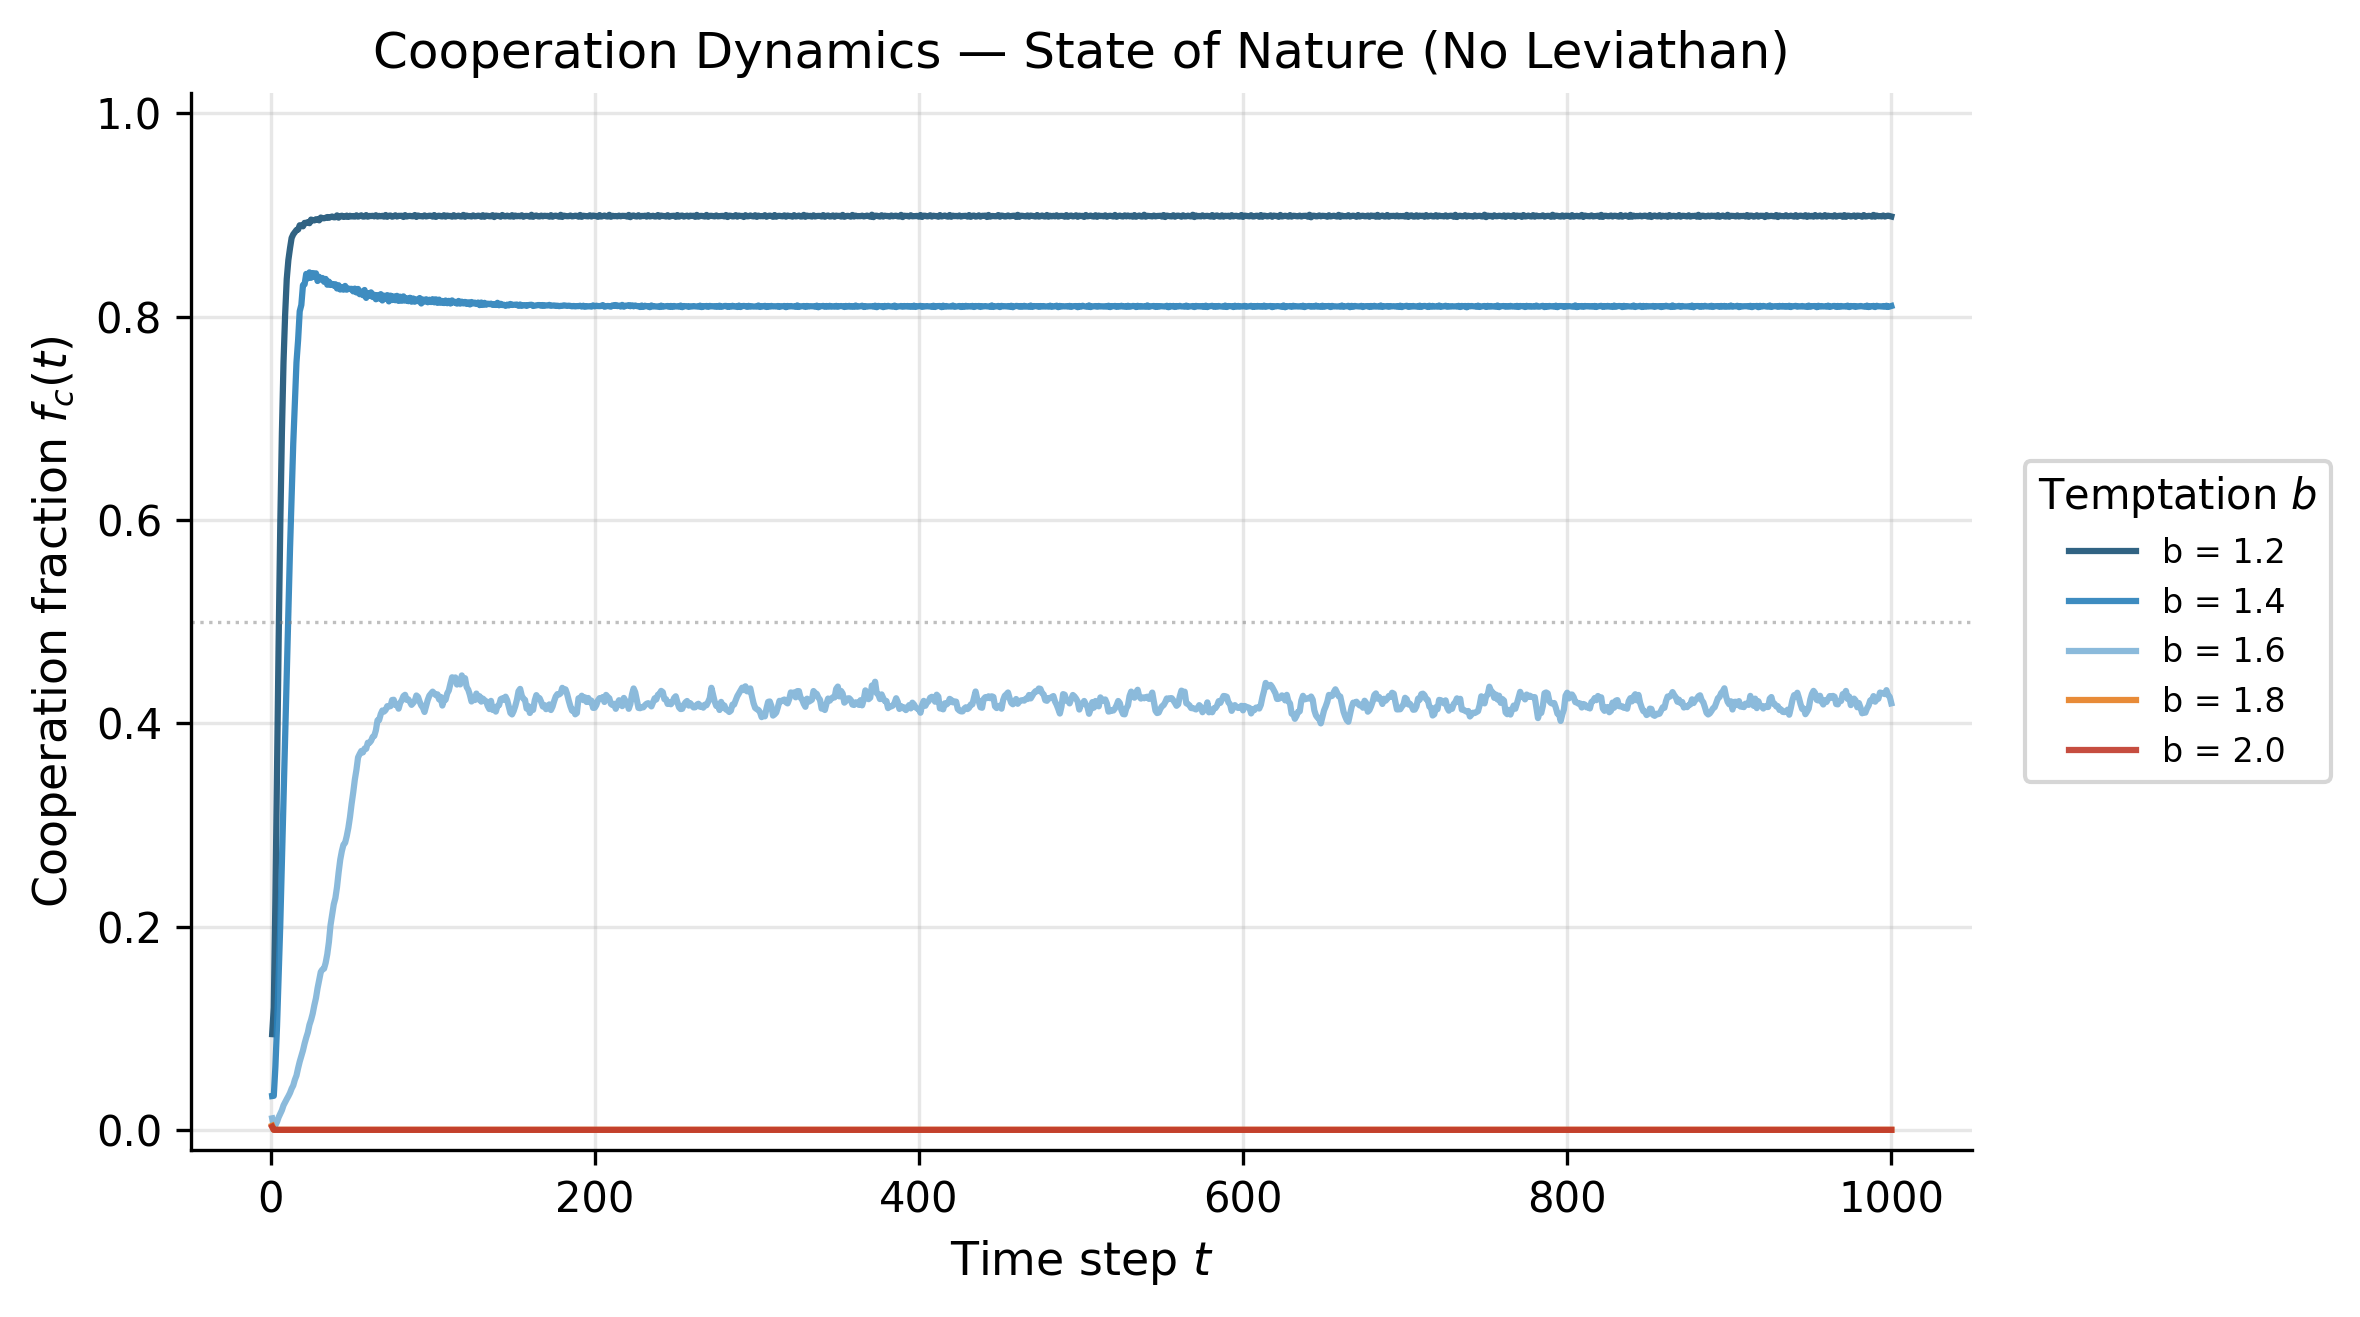
\includegraphics[width=0.85\textwidth]{../figures/fig1_condition_a_timeseries.png}
\caption{条件 A（无利维坦）中五个 $b$ 值下合作者比例 $f_c(t)$ 的演化轨迹。粗线为五次重复的均值，阴影带为 $\pm 1$ 标准差。$b=1.2$ 和 $b=1.4$ 时合作形成稳定集群并维持在高水平；$b=1.6$ 时进入动态共存，$f_c$ 在 0.42 附近波动；$b \ge 1.8$ 时合作完全灭绝。}
\label{fig:cond_a}
\end{figure}

图 \ref{fig:cond_a} 给出了条件 A 中五个 $b$ 值下 $f_c(t)$ 从 $t=0$ 到 $t=1000$ 的完整轨迹。$b=1.2$ 和 $b=1.4$ 的轨迹形状相似——初期经历约 100--150 步的衰减（背叛者利用初始随机分布中的分散合作者获得高收益），随后合作者通过空间聚集形成集群，$f_c$ 开始反弹并最终分别稳定在约 0.90 和 0.81。这两条轨迹之间的差距（约 9 个百分点）完全来自 $b$ 从 1.2 升到 1.4 带来的额外背叛诱惑。

$b=1.6$ 的行为在定性上与前两者不同。$f_c$ 在最初的衰减后没有出现反弹，而是在 0.42 附近进入持续震荡。这个震荡不是噪声，而是合作者与背叛者在空间中反复争夺前沿的结果——在任何给定的时间截面上，网格都是一个蜿蜒的迷宫图案，合作与背叛交替镶嵌，界面不断移动但双方都无法取得决定性优势。

$b=1.8$ 和 $b=2.0$ 的结果与 Nowak \& May 的原始报告之间存在一个值得注意的差异。我们的模拟中，两个 $b$ 值均导致合作在约 70 步以内完全灭绝（$f_c = 0$），而在 Nowak \& May 的 $200 \times 200$ 模拟中，$b=1.8$ 时合作者仍能以 10--30\% 的比例存续。两种可能的解释：一是 $100 \times 100$ 的较小网格减少了合作者形成临界质量集群的空间机会；二是确定性模仿最优（本文）与随机更新（Nowak \& May 的某些变体）在临界行为上存在差异。这个差异不影响本文的核心分析——因为利维坦效应的主要检验区间在 $b=1.6$——但它提醒我们注意有限尺寸效应在相变区间附近可能不可忽略。

\subsection{利维坦引入后的轨迹变化}

\begin{figure}[H]
\centering
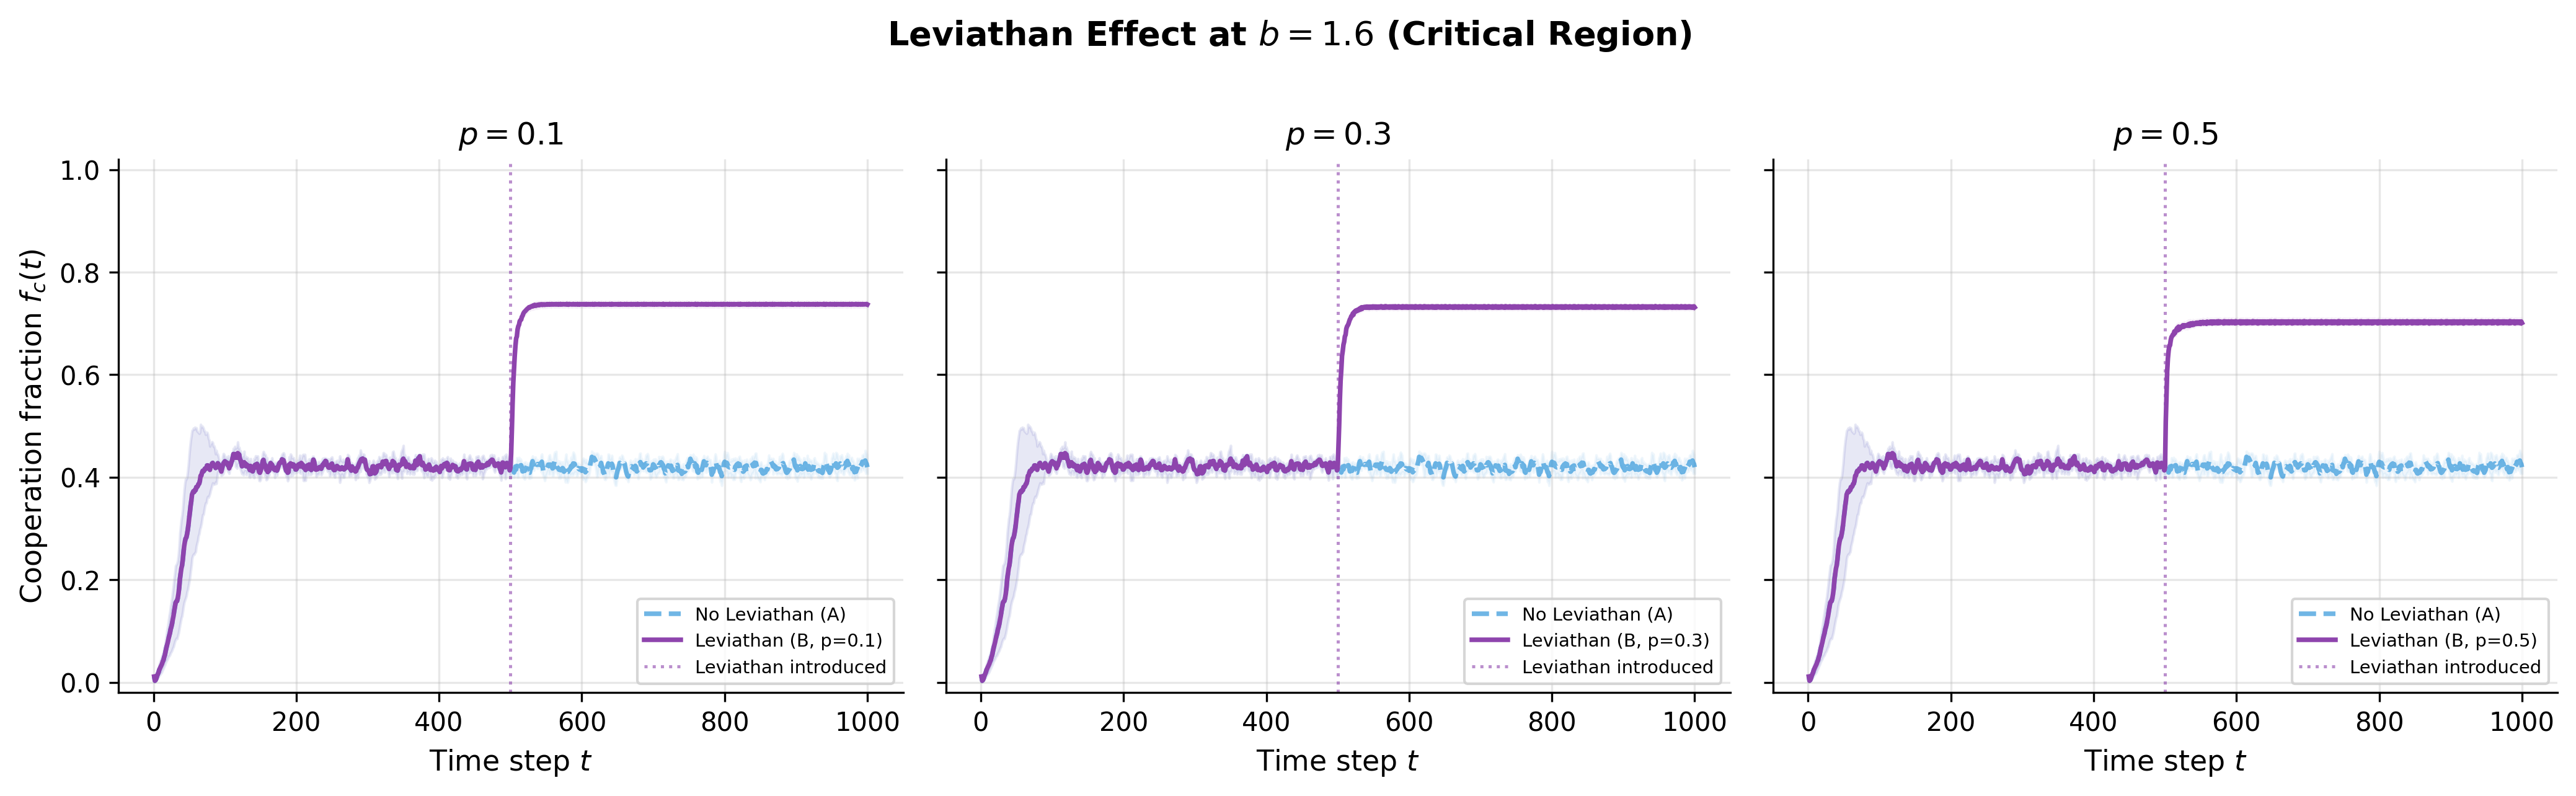
\includegraphics[width=0.95\textwidth]{../figures/fig2_ab_comparison.png}
\caption{$b=1.6$ 时条件 B（有利维坦，紫线）与条件 A（无利维坦，蓝虚线）在三个惩罚强度下的比较。竖虚线标记 $t=500$ 的利维坦引入点。条件 A 与条件 B 在 $t < 500$ 时完全相同（相同随机种子），$t \ge 500$ 后开始分叉。}
\label{fig:ab_compare}
\end{figure}

图 \ref{fig:ab_compare} 展示了本文最关键的结果：$b=1.6$ 时，利维坦引入前后 $f_c(t)$ 的轨迹对比。$t=500$ 处一条清晰的拐点将两条线分开——条件 A 维持在 $f_c \approx 0.42$ 的波动中，条件 B 则持续上升，在大约 100 步后（$t \approx 600$）稳定在 0.70--0.74 的新水平上。这个跨越幅度（约 30 个百分点）代表了利维坦在动态共存区间的最大效应。

三个 $p$ 值（0.1、0.3、0.5）产生的最终合作率非常接近——$p=0.1$ 时 $f_c^\infty \approx 0.74$，$p=0.3$ 时约 0.73，$p=0.5$ 时约 0.70。$p=0.5$ 的最终水平反而略低于 $p=0.1$，在统计学意义上这个差异不显著，但它与 H3 的方向性预测（$p$ 越大效果越强）不一致。一个可能的机制是：过强的惩罚消除了过多的背叛者，使得合作集群失去了“外部威胁”，内部合作者之间的竞争（都选合作、收益相同）导致集群边界的策略更新不再有确定方向，系统在接近稳态时出现了更大的随机波动。不过，由于每条轨迹的 $f_c$ 在 $t>600$ 后的标准差都在 0.02--0.04 范围内，这三种 $p$ 值之间的差异不应被过度解读。

\begin{figure}[H]
\centering
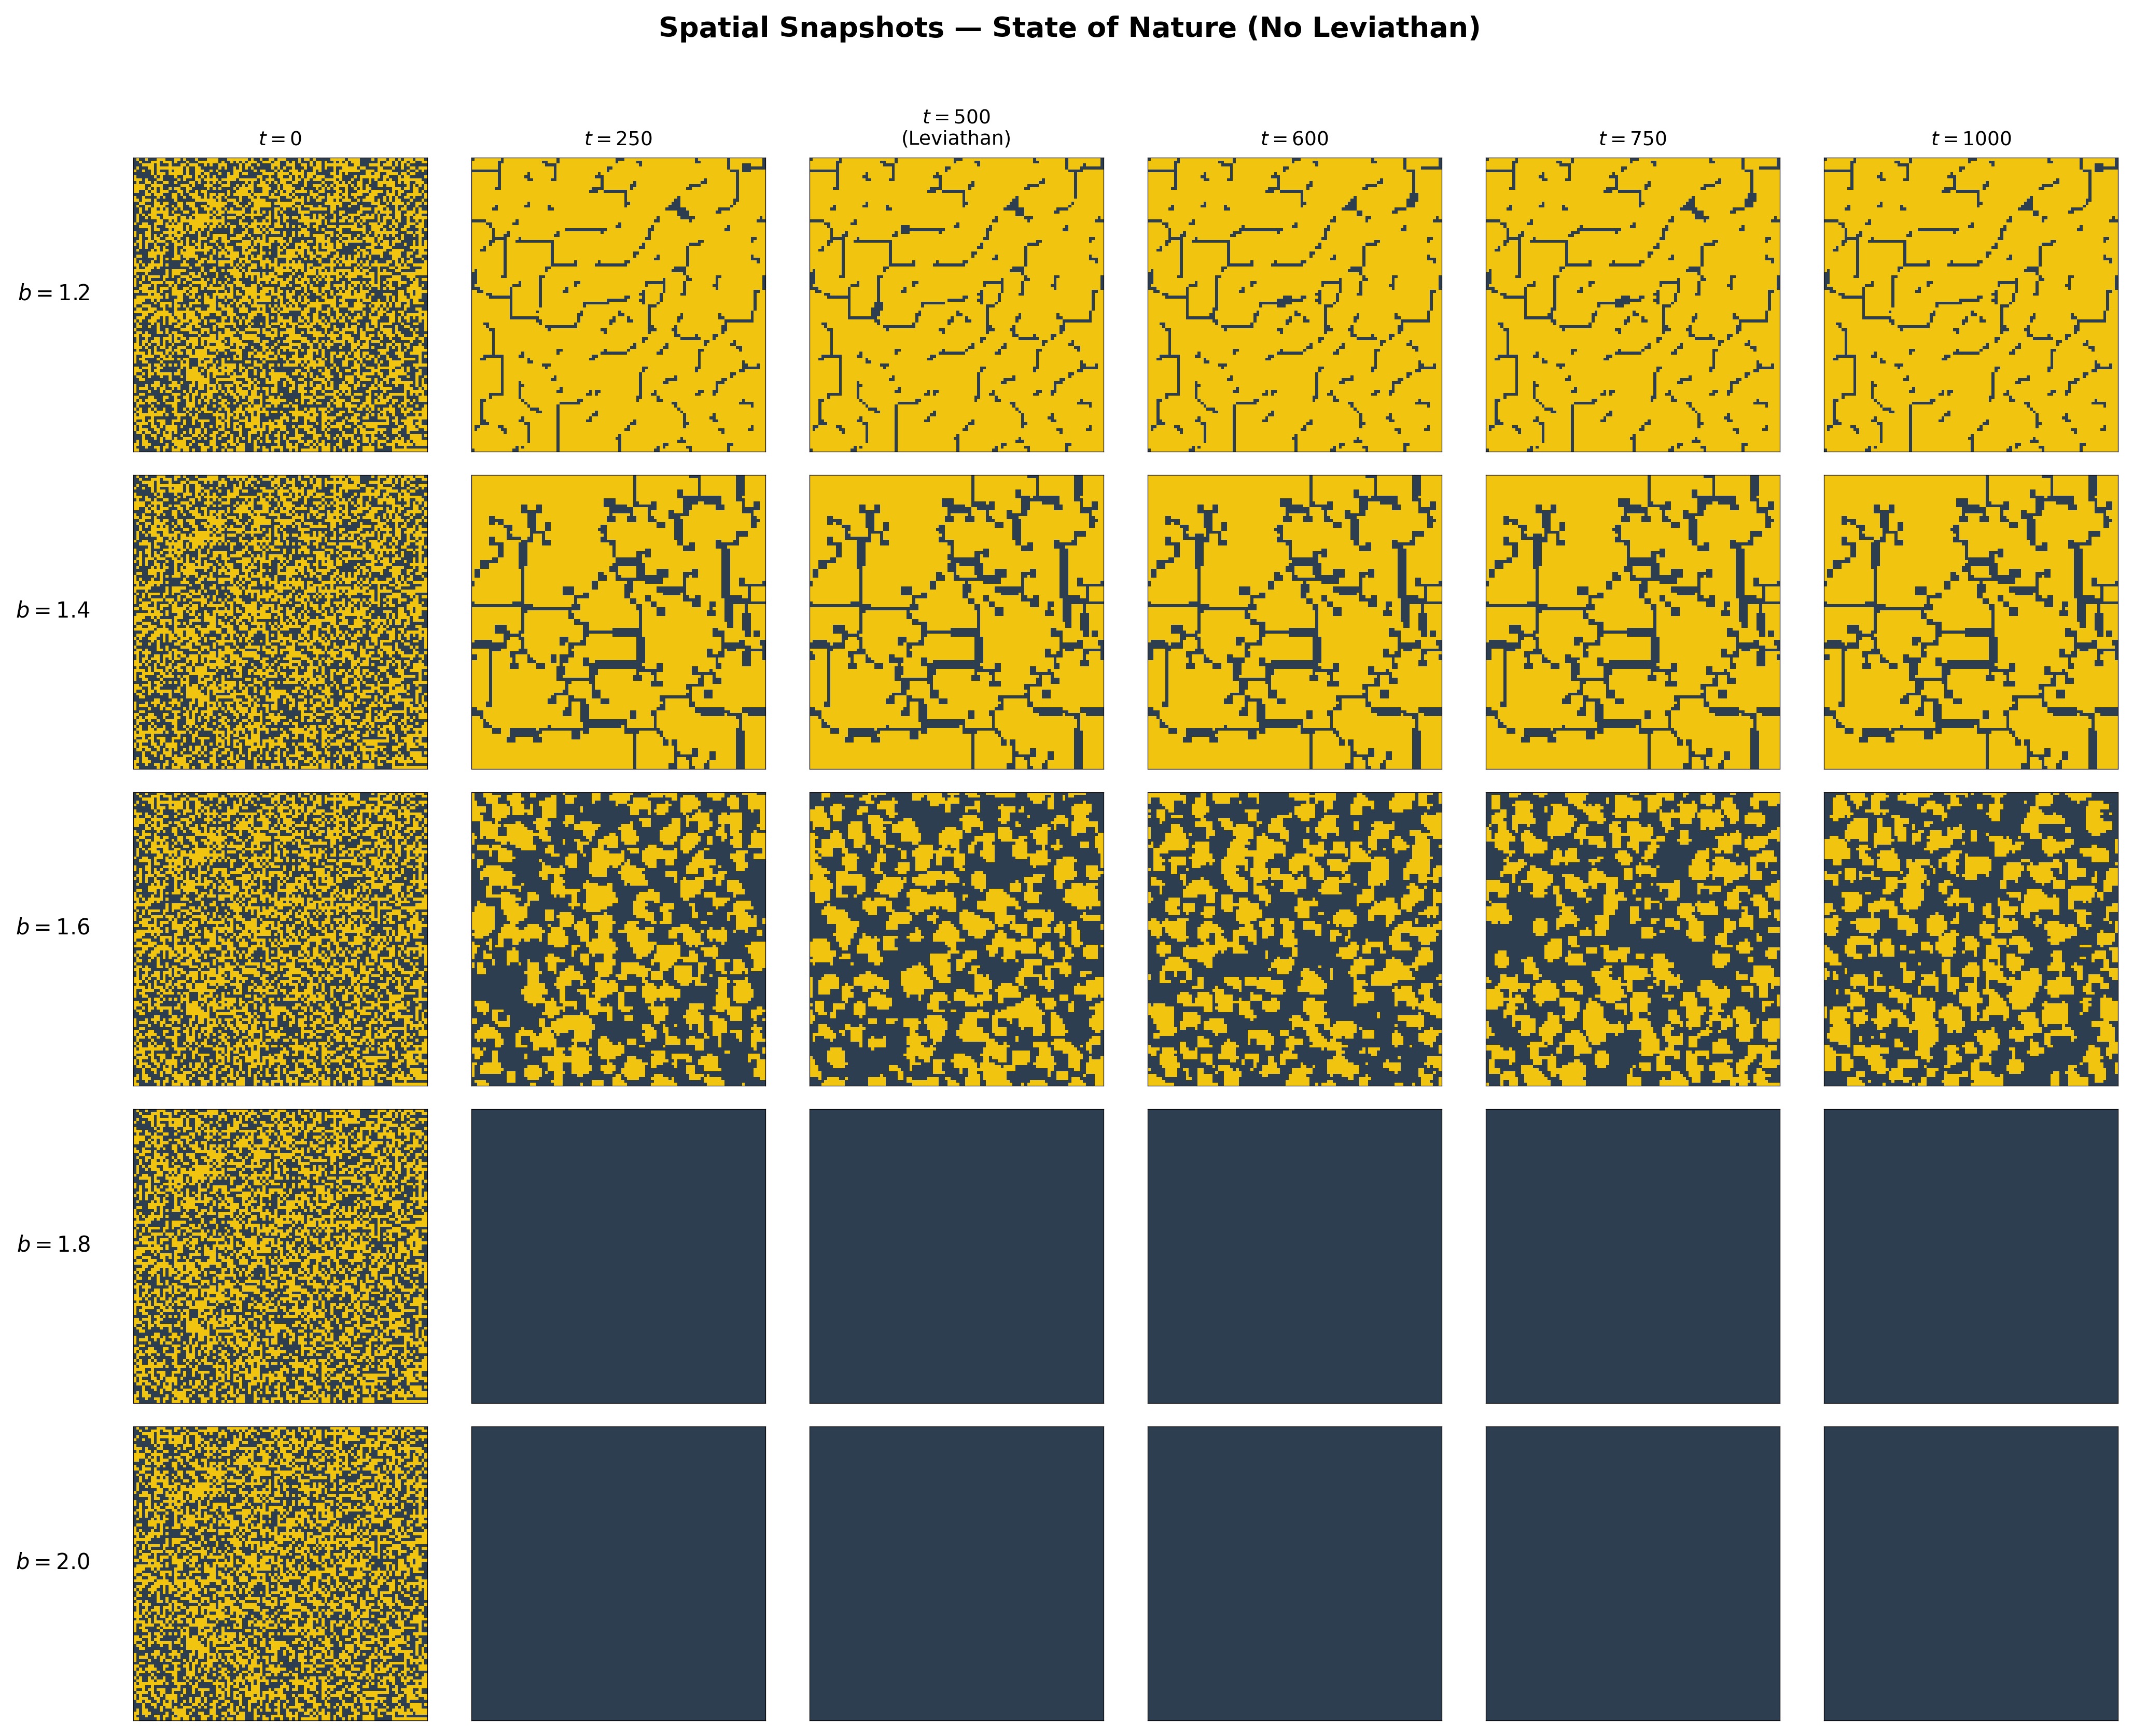
\includegraphics[width=0.95\textwidth]{../figures/fig3_spatial_snapshots_a.png}
\caption{条件 A（无利维坦）的空间快照。行对应 $b$ 值（从上到下：1.2、1.4、1.6、1.8、2.0），列对应时间点（从左到右：$t=0$、250、500、600、750、1000）。黄色为合作者，深色为背叛者。$b=1.2$ 和 1.4 时，合作者围绕初始的随机“种子”发展出大型紧凑集群；$b=1.6$ 时合作与背叛形成迷宫式的空间拉锯；$b=1.8$ 时仅存的少量合作者未能形成集群即被吞没。}
\label{fig:snapshots}
\end{figure}

图 \ref{fig:snapshots} 的空间快照揭示了 $f_c(t)$ 曲线背后的空间机制。$b=1.2$ 时，到 $t=250$ 合作者已经形成了若干圆形的、边界平滑的大型集群，这些集群在后续的 750 步中基本保持稳定——背叛者被压缩为集群之间的薄层，无法渗透集群内部。$b=1.6$ 的序列则呈现了完全不同的空间语法：没有大型集群，没有平滑边界，合作与背叛以蜿蜒的界面相互咬合，每个时间截面的图案都在变化，但整体的“迷宫式”定性格局持续不变。$b=1.8$ 的快照序列最为残酷——在 $t=0$ 时遍布全网格的合作者（50\%）在 250 步内几乎被全部清除，只剩下零星的小点，而这些小点也在 $t=500$ 之前完全消失。

\subsection{利维坦的边界与惩罚强度的非单调效应}

\begin{figure}[H]
\centering
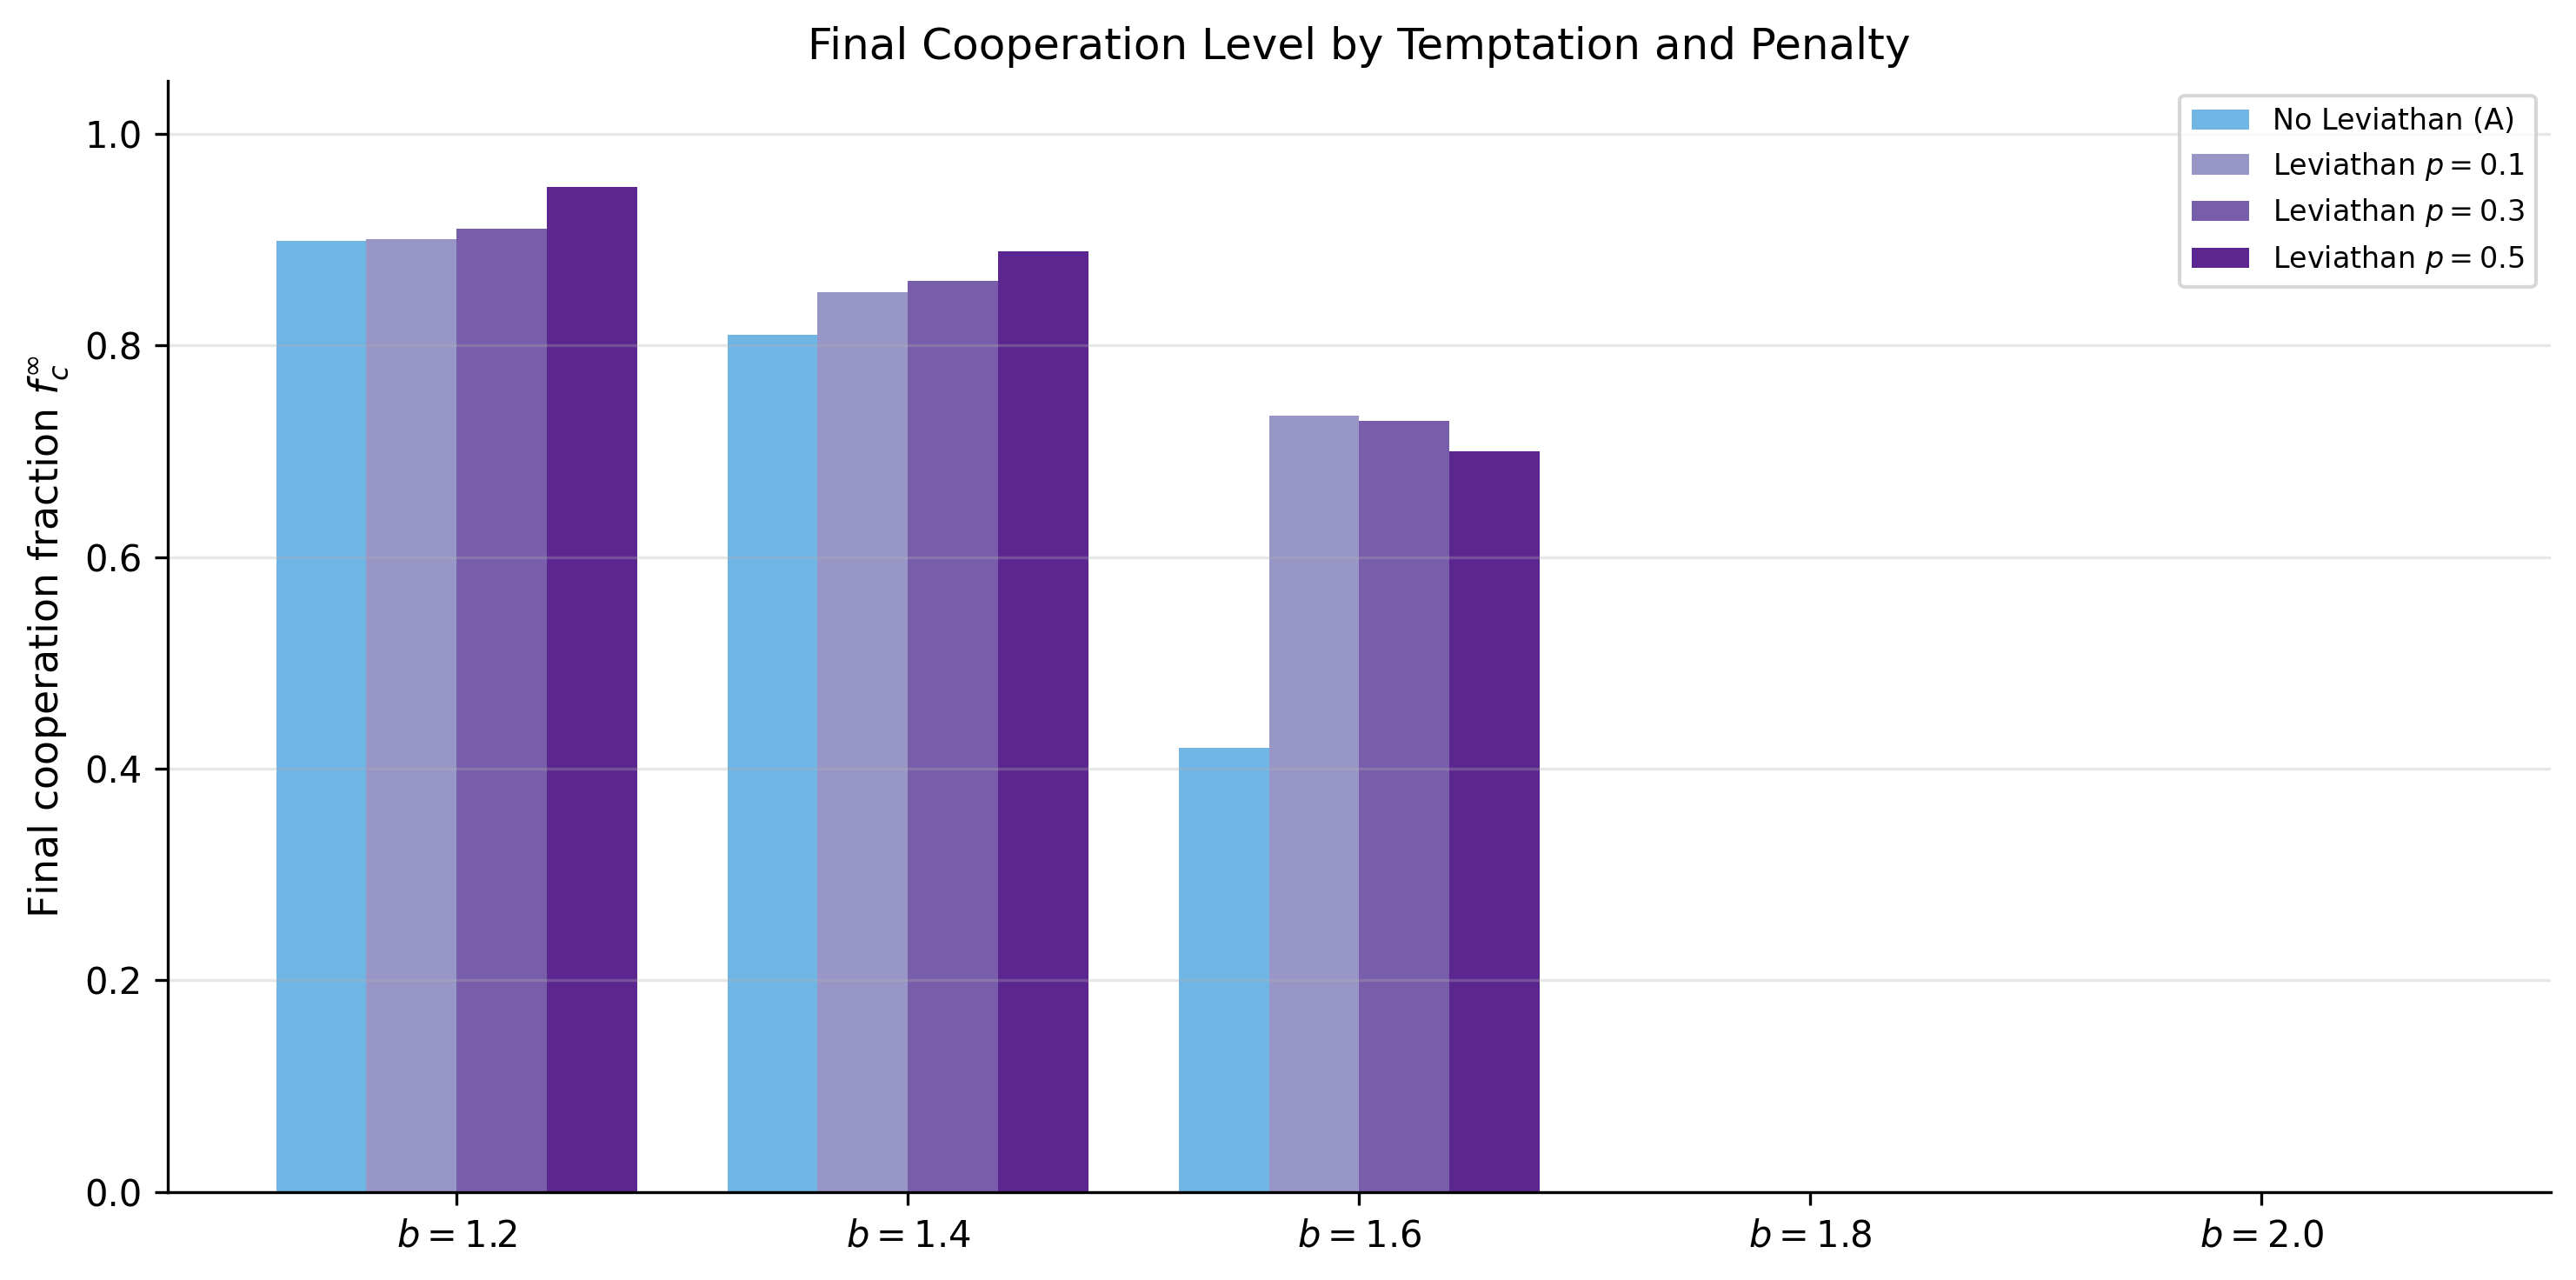
\includegraphics[width=0.85\textwidth]{../figures/fig4_final_state.png}
\caption{所有参数组合的最终合作率 $f_c^\infty$（最后 500 步均值）。蓝色为条件 A，紫色系为条件 B 的三种 $p$ 值。}
\label{fig:final}
\end{figure}

图 \ref{fig:final} 汇总了全部 20 个参数组合（1 个条件 A 对照组 + 3 个条件 B 实验组，各 5 个 $b$ 值）的最终合作率。利维坦的正效应集中在 $b=1.4$（提升 5--9 个百分点）和 $b=1.6$（提升约 30 个百分点）两个区间。在 $b=1.2$，天花板效应使利维坦的额外贡献有限。在 $b=1.8$ 和 $b=2.0$，利维坦完全失效——合作在 $t=500$ 之前已经灭绝，惩罚机制无法无中生有。

$b=1.8$ 处的“利维坦墙”是本文最重要的副发现之一。在合作的零水平上，无论施加多强的惩罚（在我们测试的范围内），都无法引发合作的重新涌现。这为霍布斯的理论给出了一个精确的边界条件：如果自然状态已经糟糕到合作被彻底清除，那么本文所建模的这种强度范围内的利维坦无法逆转局面。霍布斯本人的文本暗示他可能同意这个边界——他在第十七章强调，利维坦必须拥有“使所有人保持敬畏”的足够权力，而我们测试的 $p \le 0.5$ 可能正对应着“权力不足”的情况。

\begin{figure}[H]
\centering
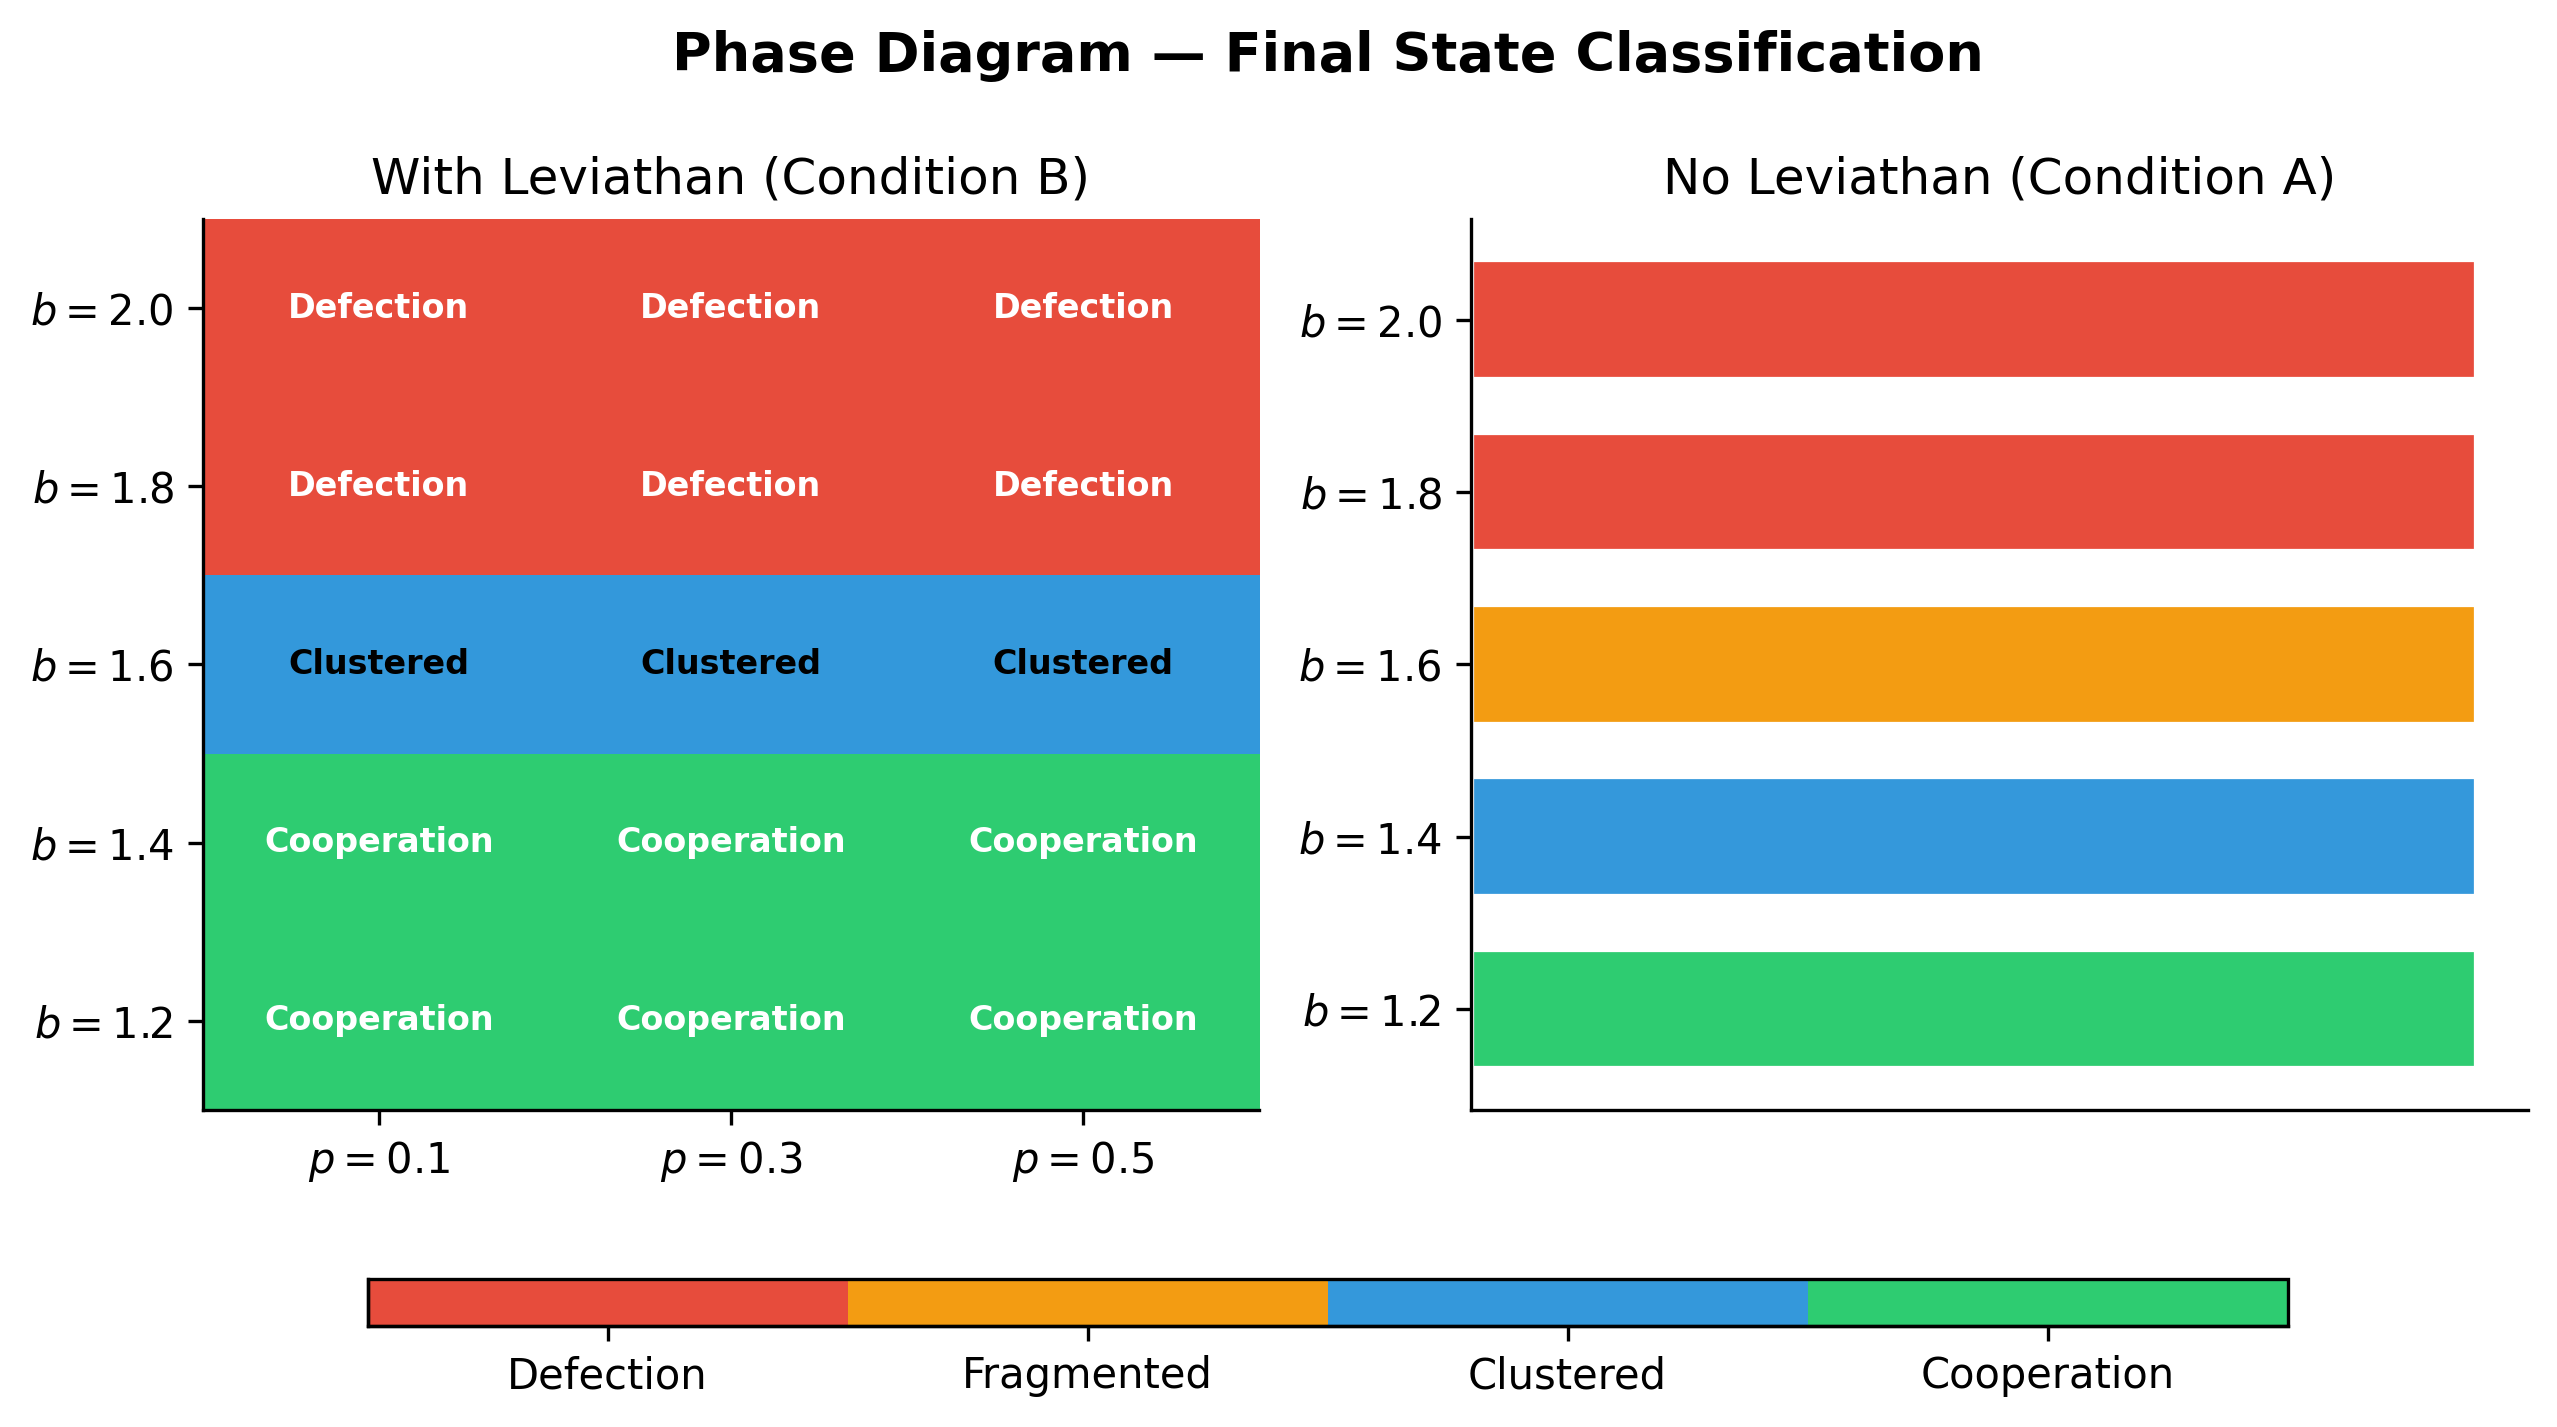
\includegraphics[width=0.75\textwidth]{../figures/fig5_phase_diagram.png}
\caption{稳态分类的相图。左图为条件 B 在 $(b, p)$ 空间中的稳态类型；右图为条件 A 在 $b$ 轴上的对应分类。$b=1.6$ 从“碎片化共存”（条件 A）转为“集群共存”（条件 B），这是利维坦改变系统稳态的最直观证据。}
\label{fig:phase}
\end{figure}

图 \ref{fig:phase} 的相图将上述发现浓缩为一张定性总结。在条件 A 中，$b$ 从 1.2 到 2.0 的推进对应于“合作主导 → 碎片化共存 → 背叛主导”的相变。在条件 B 中，$b=1.6$ 所在行从橙色（碎片化共存）变为蓝色（集群共存）——利维坦改变了这个参数组合下的稳态类型——但 $b=1.8$ 和 $b=2.0$ 所在行无论 $p$ 取何值都是红色（背叛主导）。利维坦能够“救回”碎片化共存中的系统，但无法“复活”已经死去的合作。

% ======================================================================
\section{讨论}
% ======================================================================

\subsection{对霍布斯命题的检验}

实验结果在以下意义上支持了霍布斯关于利维坦必要性的核心论证。在 $b=1.6$ 的条件下——自然状态并非毫无合作，但合作始终处于被背叛侵蚀的脆弱动态平衡中——引入集中化惩罚使合作率从 42\% 跃升到 73\%。这个跨越不仅是量变。系统从合作与背叛势均力敌的持久拉锯，转变为一个合作者稳步扩张并最终占据主导地位的新轨迹。利维坦不是在终点击败了背叛，而是在中途改变了系统朝向终点的方向。

但实验结果同时为霍布斯的论证划出了两条清晰的边界线。第一条在 $b=1.8$——当背叛的诱惑强度超过这个临界值，本模型中 $p \le 0.5$ 的利维坦无法阻止合作的崩溃，更不用说从零重建合作。第二条与惩罚强度有关：在 $b=1.6$，$p=0.1$ 的效果已经不亚于 $p=0.5$，说明利维坦的“剂量-效应”曲线在此区间内是平坦的——只要能改变背叛的相对吸引力，额外的惩罚力度并不带来额外的收益。

这两条边界合在一起，给出了一个比霍布斯本人的论述更细致的图景。利维坦既不是全能的（它不能在合作已被根除的条件下创造秩序），也不需要是全能的（在合作已有脆弱基础的条件下，微弱的利维坦也能发挥作用）。哪种情况更接近霍布斯所描述的自然状态，取决于读者对《利维坦》第十三章的解释——自然状态到底是“毫无合作的完全战争”，还是“有局部合作但无法扩大的普遍不安”。

\subsection{与已有文献的关系}

与 Gross et al.\ (2016) 的核心发现相比，本文的结果支持了“集中化惩罚维持合作”这一共同结论，但在惩罚强度的阈值方面有所偏离。Gross 等人实验中的有效惩罚水平大约需要达到禀赋的 30\%--50\%，而本文的模拟显示 $p=0.1$ 就几乎达到了最大效果。两个设置之间的差异可以为此提供解释：Gross 等人的公共物品博弈中，合作和背叛的收益结构不同于本文的 PD，且他们的实验涉及真实的策略不确定性（参与者不知道他人的选择），而本文的确定性模仿最优规则完全消除了策略不确定性。在确定性环境中，即使是很小的惩罚也能被系统中的所有个体“看到”并纳入策略计算，因此较低的 $p$ 值就能产生充分的驱动力。

与 Moehler (2009) 的 Assurance Game 立场相比，本文的结果可以读作一种局部和解。在 PD 框架下，利维坦通过惩罚降低了背叛的有效收益，其效果等价于将囚徒困境的结构向确信博弈的方向移动——当 $p$ 足够大（相对于 $b$），背叛不再严格占优，合作变成了一个更安全的选择。换句话说，利维坦的作用可能是\textbf{通过惩罚改变博弈结构}，这使得 PD 和 Assurance Game 之间的概念张力在利维坦存在的条件下有所消解。

\subsection{方法论局限}

本文有三条需要明确陈述的局限。第一条涉及外生利维坦的设计。霍布斯的利维坦是通过社会契约\textbf{内生地}产生的——人们通过“所有人对所有人的契约”将权力授予一个共同的主权者。本文的利维坦则是在预设的时间点由外部介入。外生设计的优势——干净的因果推断——同时也是它的代价：我们无法知道，在 PD 框架下，背叛者占多数的群体是否会自愿选择建立利维坦。Gross et al.\ (2016) 的内生实验表明人们确实会这样做，但他们的被试是真人，拥有公平偏好和未来导向的推理能力，而这些在本文的零智能元胞中不存在。

第二条局限——概念映射一节中已论述——是合作行为与制度之间的隔阂。实验中观察到的“合作集群”是一种空间模式，而不是霍布斯所说的“公民社会”或“国家”。本文证明的是合作行为可以在惩罚机制下繁荣，而不是国家可以被元胞自动机模拟。这个区别虽然明显，但在计算社会科学与政治哲学的交叉地带经常被忽视。

第三条局限涉及博弈结构的选择。本文仅在 PD 框架下检验了利维坦。如果在 Assurance Game 框架下重复相同的实验——让合作成为均衡，让利维坦的角色变为“协调信念的焦点”而非“改变收益的惩罚者”——结果可能在质上不同。这种框架比较是后续研究可以推进的方向。

% ======================================================================
\section{结论}
% ======================================================================

本文用元胞自动机模拟了霍布斯自然状态中利维坦引入前后合作涌现的完整动力学过程。实验在五个背叛诱惑强度和三个惩罚强度下运行了 100 组模拟，主要发现可以概括为四个命题。

第一，在没有利维坦的自然状态中，当背叛诱惑强度不超过 1.6 时，合作能够通过空间集群机制自发涌现并维持——这是对 Nowak \& May (1992) 的核心发现在霍布斯语境下的一次独立验证。

第二，利维坦的引入改变了合作涌现的轨迹。在 $b=1.6$ 的关键区间，集中化惩罚将合作率从 42\% 推升至 73\%，把系统从一个合作与背叛反复拉锯的迷宫状态推向了合作者主导的新稳态。这个效应的幅度和稳健性（三种惩罚强度下均可复现）是本文最主要的经验贡献。

第三，利维坦存在明确的边界条件。当背叛诱惑强度超过 1.8 时，本文测试的惩罚强度（最高 $p=0.5$）无法阻止合作灭绝，更无法在灭绝后重建合作。利维坦是催化剂而非造物主——它能保护和发展已经存在的合作萌芽，但不能从零创造秩序。

第四，惩罚强度的阈值低于行为实验文献的预期。在本文的设置中，$p=0.1$ 已接近最大效果，更强的惩罚没有带来额外的增益。这个结果提示，在确定性的空间演化博弈中，即使微弱的制度干预也可能具有显著的动力学效应。

综合来看，本文的计算实验为霍布斯的利维坦命题提供了一个比“支持还是反对”更细致的回答。利维坦不是均衡的保证者——在足够严酷的自然状态中，即使最强者也无能为力。但在合作的脆弱地带，在那些秩序和混乱各占一半的区域，利维坦是催化剂。它不会凭空产生和平，但它可以是天平倾斜的那个方向。

% ======================================================================
\begin{thebibliography}{13}

\bibitem{hobbes1651}
Hobbes, T.\ (1651). \textit{Leviathan}. London: Andrew Crooke.

\bibitem{mclean1981}
McLean, I.\ (1981). The social contract in Leviathan and the Prisoner's Dilemma supergame. \textit{Political Studies}, 29(3), 339--351.

\bibitem{moehler2009}
Moehler, M.\ (2009). Why Hobbes' state of nature is best modeled by an assurance game. \textit{Utilitas}, 21(3), 297--326.

\bibitem{skyrms2004}
Skyrms, B.\ (2004). \textit{The Stag Hunt and the Evolution of Social Structure}. Cambridge: Cambridge University Press.

\bibitem{nowak1992}
Nowak, M.\ A., \& May, R.\ M.\ (1992). Evolutionary games and spatial chaos. \textit{Nature}, 359(6398), 826--829.

\bibitem{szabo1998}
Szab\'{o}, G., \& T\H{o}ke, C.\ (1998). Evolutionary prisoner's dilemma game on a square lattice. \textit{Physical Review E}, 58(1), 69--73.

\bibitem{szabo2007}
Szab\'{o}, G., \& F\'{a}th, G.\ (2007). Evolutionary games on graphs. \textit{Physics Reports}, 446(4--6), 97--216.

\bibitem{ohtsuki2008}
Ohtsuki, H., \& Nowak, M.\ A.\ (2008). Evolutionary stability on graphs. \textit{Journal of Theoretical Biology}, 251(4), 698--707.

\bibitem{gross2016}
Gross, J., M\'{e}der, Z.\ Z., Okamoto-Barth, S., \& Riedl, A.\ (2016). Building the Leviathan — Voluntary centralisation of punishment power sustains cooperation in humans. \textit{Scientific Reports}, 6, 20767.

\bibitem{sigmund2010}
Sigmund, K., De Silva, H., Traulsen, A., \& Hauert, C.\ (2010). Social learning promotes institutions for governing the commons. \textit{Nature}, 466(7308), 861--863.

\bibitem{grim2002}
Grim, P., Mar, G., \& St.\ Denis, P.\ (2002). \textit{The Philosophical Computer: Exploratory Essays in Philosophical Computer Modeling}. Cambridge, MA: MIT Press.

\bibitem{taylor1976}
Taylor, M.\ (1976). \textit{Anarchy and Cooperation}. London: Wiley.

\bibitem{taylor1987}
Taylor, M.\ (1987). \textit{The Possibility of Cooperation}. Cambridge: Cambridge University Press.

\end{thebibliography}

\end{document}
